\documentclass[12pt]{article}
\usepackage{graphicx}
\usepackage{float}
\usepackage{caption}
\usepackage{subcaption}
\usepackage{fullpage}
\usepackage{lastpage}
\usepackage{fancyhdr}
\usepackage{wrapfig}
\usepackage{lipsum}
\usepackage{mathtools}
\usepackage{amsfonts}
\usepackage{enumitem}
\usepackage{amsmath}
\usepackage{listings}
\usepackage[margin=0.8in]{geometry}

\newcommand{\s}{\hspace{5pt}}
\newcommand{\half}{\frac{1}{2}}
\newcommand{\R}{\mathbb{R}}
\newcommand{\C}{\mathbb{C}}
\newcommand{\p}{\partial}
\newcommand{\mb}{\mathbf}

\newenvironment{m}{\begin{pmatrix}}{\end{pmatrix}}
\newenvironment{e}{\begin{enumerate}[label=(\alph*)]}{\end{enumerate}}

\setlength{\parindent}{0in}

\begin{document}
	
\title{\vspace{-5ex}Plasma Educational Notes: Langmuir Waves\vspace{-1ex}}
\date{\vspace{-1ex}\today}
\author{Kyle Miller \& Lance Hildebrand}
\maketitle

\section*{Introduction}
Waves are a fundamental collective process in plasmas. The plasma state is rich in wave phenomena. One of the basic properties of plasmas, charge neutrality, is mediated by Langmuir waves. In most plasmas of interest, the ions are much heavier than the electrons and thus the ions move little compared to the electrons. When the electrons are displaced, an electric field develops to maintain charge neutrality, which accelerates the electrons back towards the ions. The electrons will overshoot and effectively slosh around the stationary ions. These oscillations are known by a variety of names: Langmuir oscillations, space charge waves, or simply plasma oscillations. For a stationary cold plasma, there are non-propagating modes at the plasma frequency. These modes become propagating modes when the plasma drifts at a constant speed. These can be studied in the fluid description if we choose an equation of state, i.e., if we have a model for pressure as a function of density and temperature.

\section*{Dispersion Relation}
We consider a plasma with warm electrons and cold ions. First we choose the ideal equation of state, $P=\gamma \tilde{n}_e T_e$, where $\gamma \approx 3$ is the adiabatic index obtained from kinetic theory. We can then write the five linearized fluid equations. First we have the Navier-Stokes equations for both the electrons and ions, respectively:
\[
	\begin{dcases}
		\frac{\p}{\p t}\tilde{\mb{v}}_e=-\frac{e}{m_e}\tilde{\mb{E}}-\frac{\gamma T_e}{m_e n_{0e}}\nabla \tilde{n}_e\\
		\frac{\p}{\p t} \tilde{\mb{v}}_i=\frac{Ze}{m_i}\tilde{\mb{E}}.
	\end{dcases}
\]
The continuity equations are
\[
	\begin{dcases}
		\frac{\p}{\p t}\tilde{n}_e+\nabla \cdot [n_{0e}\tilde{\mb{v}}_e]=0\\
		\frac{\p}{\p t}\tilde{n}_i+\nabla \cdot [n_{0i}\tilde{\mb{v}}_i]=0,
	\end{dcases}
\]
and finally Poisson's equation is given as
\[
	\nabla \cdot \tilde{\mb{E}}=-4 \pi e (\tilde{n}_e-Z\tilde{n}_i).
\]
We then take the divergence of the Navier-Stokes equations and the time derivative of the continuity equations and combine. We then go Fourier space by assuming plane wave solutions, i.e., $\p_t \rightarrow -i\omega$ and $\nabla \rightarrow ik$. Solving the resulting equation for $\tilde{n}_e$ gives
\[
	\tilde{n}_e=\frac{-\frac{e n_{0e}}{m_e}i\mb{k}\cdot\tilde{\mb{E}}}{\omega^2-\frac{\gamma T_e k^2}{m_e n_{0e}}}
\]
We get a similar result for ions, but without the pressure term. We then substitute these into Poisson's Equation and collect terms to get
\[
	\left( 1-\frac{\omega_{pi}^2}{\omega ^2}-\frac{\omega_{pe}^2}{\omega^2-\frac{\gamma T_e k^2}{m_e n_{0e}}}\right) \mb{k}\cdot\tilde{\mb{E}}=0.
\]
Since $\nabla \cdot \tilde{\mb{D}} = \nabla \cdot (\epsilon \tilde{\mb{E}}) = \epsilon \mb{k} \cdot \tilde{\mb{E}}$, the term in parenthesis is then our dielectric constant. Setting this equal to zero gives the dispersion relation,
\[
	\omega^2=\omega_{pe}^2+\frac{\gamma T_e}{m_e} k^2,
\]
where we have neglected the ion contribution because it is small compared to the electron contribution for Langmuir waves. So we see that the pressure term provides an additional term to the dispersion relation (the stationary solution is just $\omega^2=\omega_{pe}^2$).

\begin{figure}[H]
\centering
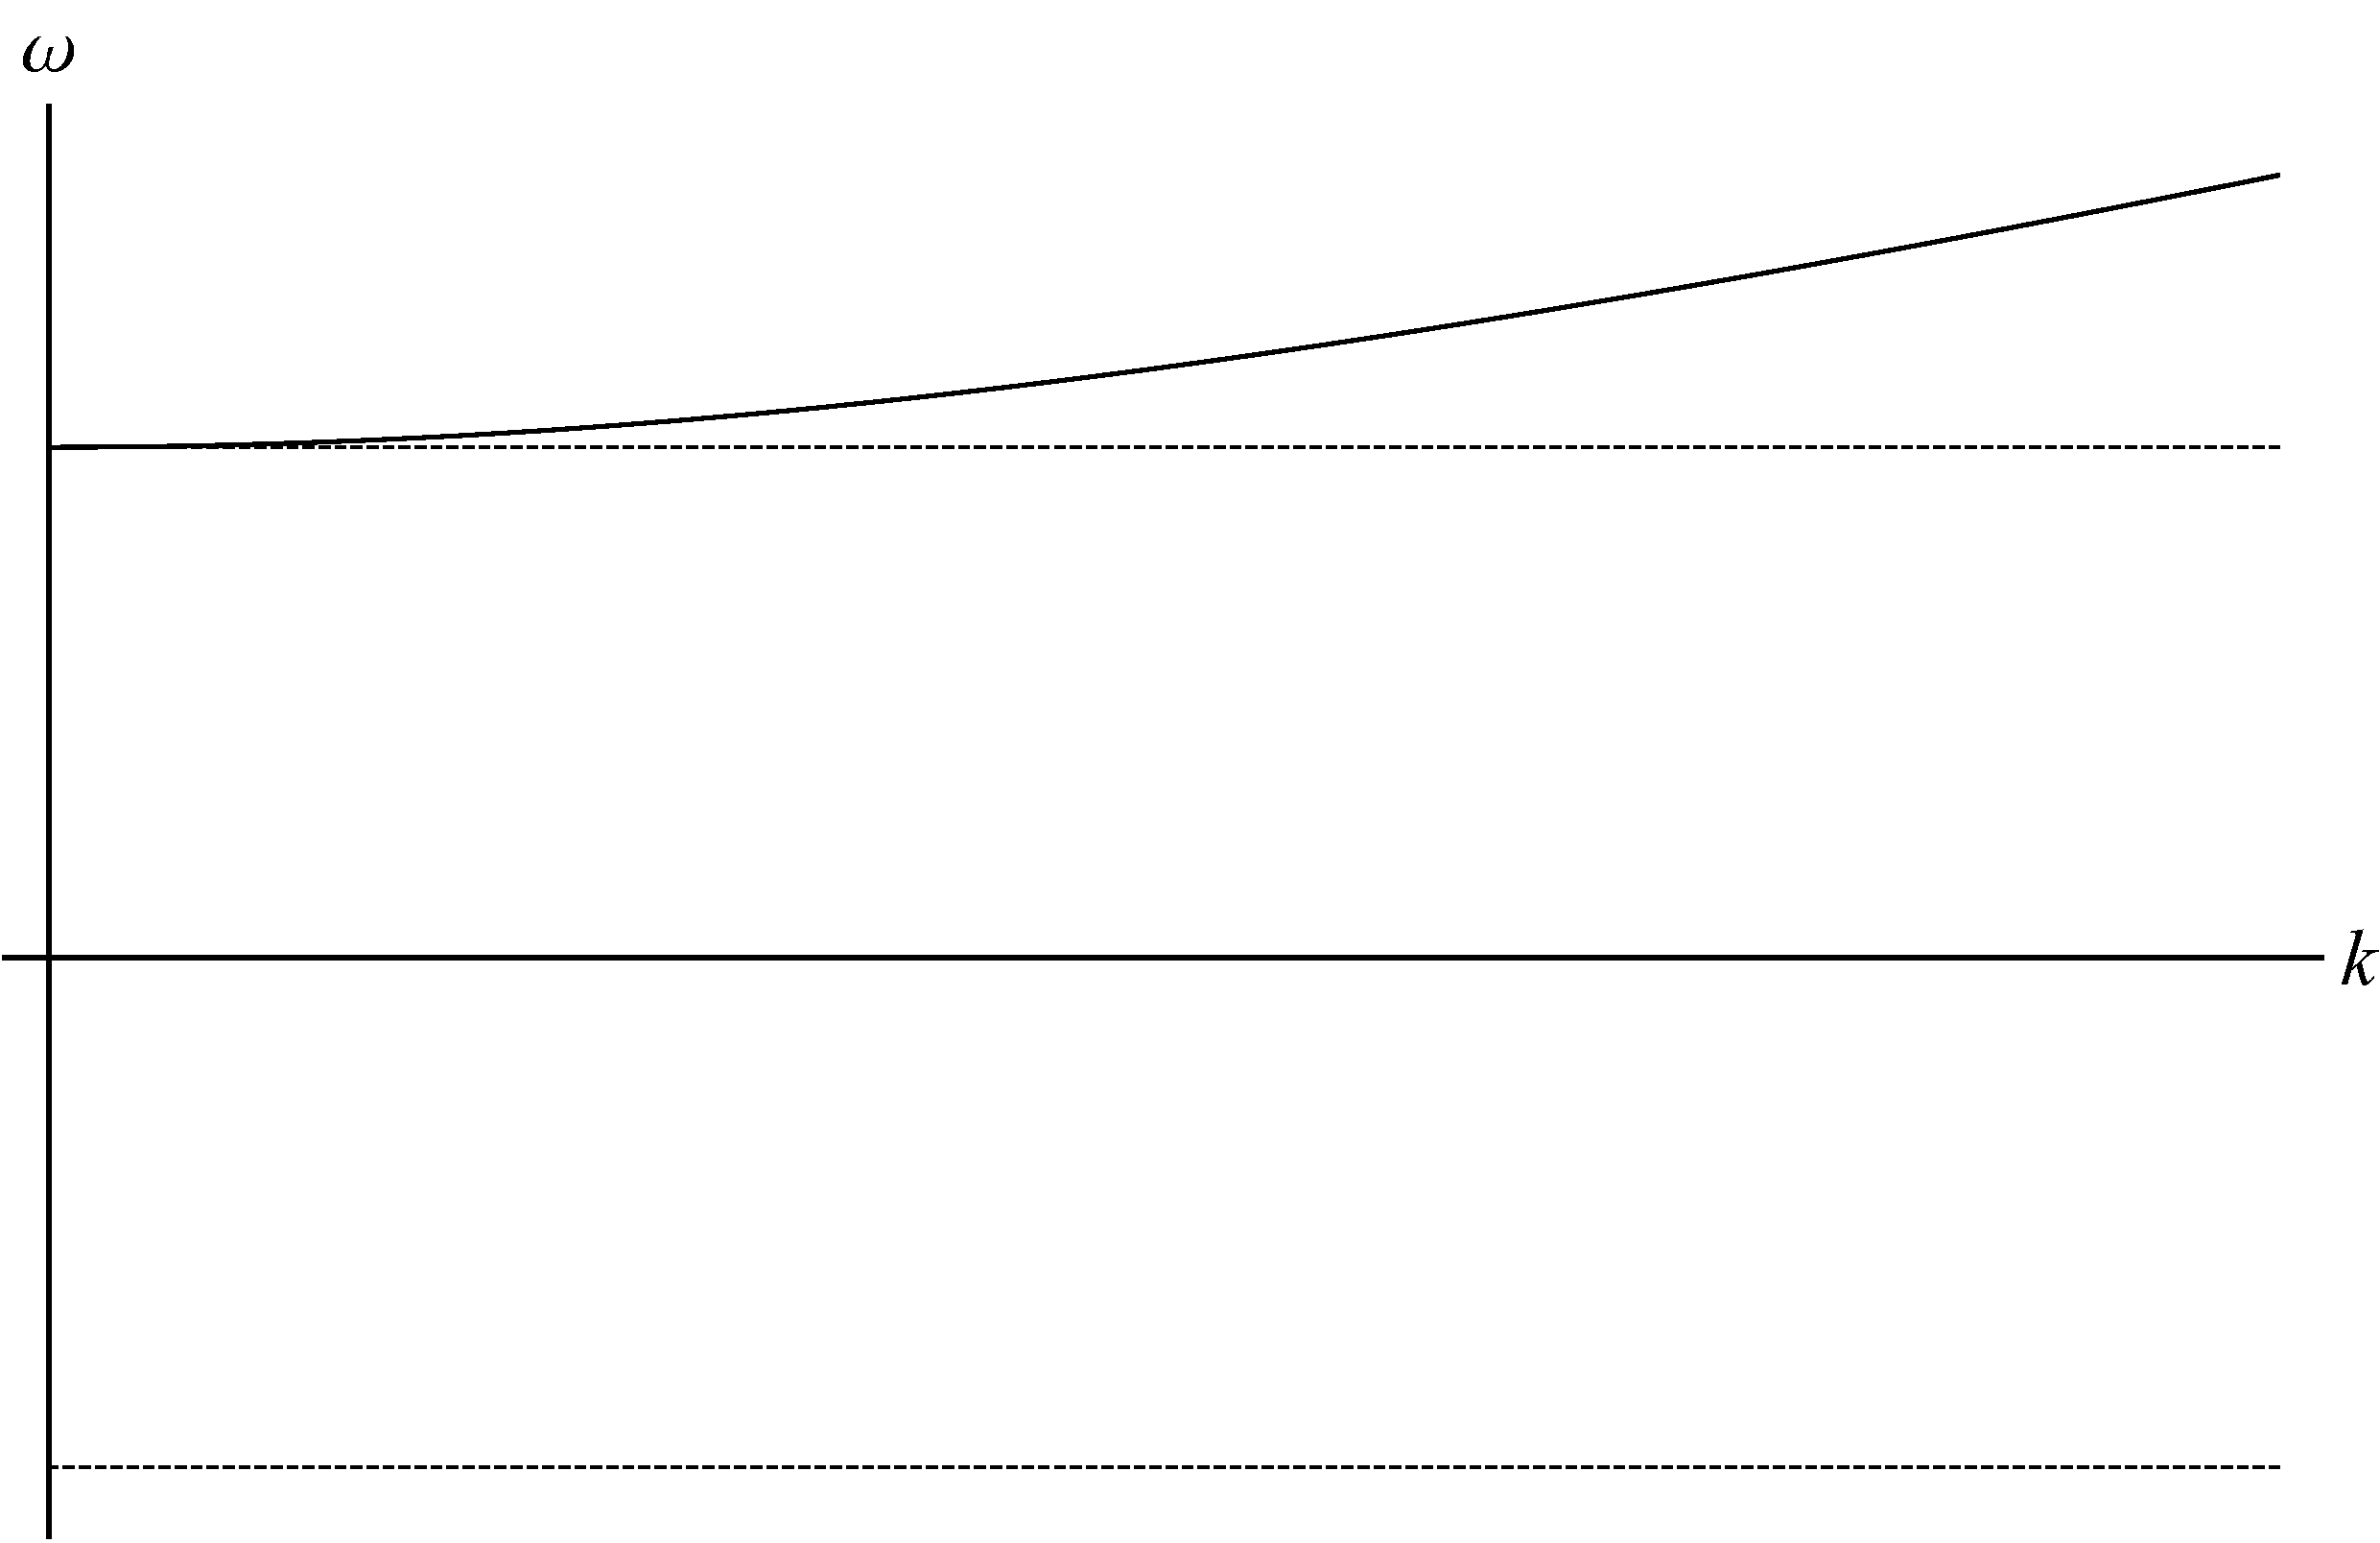
\includegraphics[width=0.5\textwidth]{langDR}
\begin{picture}(0,0)
\put(-265,112){$\omega_{pe}$}
\put(-275,5){$-\omega_{pe}$}
\end{picture}
\caption{Dispersion Relation for Langmuir Waves}
\end{figure}

\section*{Parameters}
In the dispersion relation we can substitute in the electron thermal velocity $\bar{v}_e^2=T_e/m_e$. This is now the only free parameter in the dispersion relation to vary. We can also vary the number of particles per cell to test grid stability and to see how well we conserve energy.

\section*{References}
[1] N. A. Krall and A. W. Trivelpiece, “Principle of Plasma Physics,”, pp. 143-147 McGraw Hill, New York, 1973.

\end{document}
